% Corrected for: (1) faithful float16 SOS simulation, (2) updated metrics from notebook.
% Paste into Overleaf (IEEEtran conference) or set \documentclass as in your project.
% Re-export figures from the notebook after "Run all" (includes optional \texttt{error\_psd.pdf} for diagnostics only).

\documentclass[conference]{IEEEtran}
\IEEEoverridecommandlockouts
\usepackage{cite}
\usepackage{amsmath,amssymb,amsfonts}
\usepackage{algorithmic}
\usepackage{graphicx}
\usepackage{textcomp}
\usepackage{xcolor}
\usepackage{url}
\usepackage{booktabs}

\def\BibTeX{{\rm B\kern-.05em{\sc i\kern-.025em b}\kern-.08em
    T\kern-.1667em\lower.7ex\hbox{E}\kern-.125emX}}

\begin{document}

\title{Fixed-Point vs.\ Floating-Point in IIR Filtering\\Does the Format Choice Actually Matter?}

\author{
\IEEEauthorblockN{1\textsuperscript{st} Sepehr Farrokhi}
\IEEEauthorblockA{\textit{Hanze University of Applied Sciences}\\
s.farrokhi.koochesfahani@st.hanze.nl}
\and
\IEEEauthorblockN{2\textsuperscript{nd} Amin Javan}
\IEEEauthorblockA{\textit{Hanze University of Applied Sciences}\\
ma.javan@st.hanze.nl}
\and
\IEEEauthorblockN{3\textsuperscript{rd} Armin Siavashi}
\IEEEauthorblockA{\textit{Hanze University of Applied Sciences}\\
a.siavashi@st.hanze.nl}
}

\maketitle

\begin{abstract}
When designing a DSP system, the choice between fixed-point and floating-point arithmetic directly affects accuracy, memory consumption, and hardware cost. This assignment evaluates both dimensions using a 4th-order Butterworth IIR low-pass filter as a testbed. Two fixed-point formats (Q3.13 and Q8.8) and two floating-point formats (float16 and float32) are simulated and compared against a float64 high-precision reference---not a true ground truth, but a sufficiently accurate baseline for quantifying representational error. Accuracy is measured via MSE and SNR; efficiency is assessed through memory footprint and a qualitative hardware cost analysis. The most striking finding is that format selection \emph{within} fixed-point matters greatly: Q3.13 achieves 44.87~dB SNR while Q8.8 reaches only 13.84~dB, despite identical 16-bit word length and 2000~bytes of memory. With a faithful IEEE~754 half-precision SOS simulation, float16 attains 53.68~dB SNR at the same 2000-byte signal footprint, outperforming Q3.13 yet remaining far below float32. Fixed-point offers lower hardware cost and power consumption on embedded targets; floating-point trades those efficiencies for higher precision and simpler programming where an FPU is available.
\end{abstract}

\begin{IEEEkeywords}
fixed-point, floating-point, IIR filter, quantisation error, Q-format, IEEE~754, DSP
\end{IEEEkeywords}

\section{Introduction}
Every DSP system encodes numbers in finite binary words. Whether those words use fixed-point or floating-point arithmetic determines accuracy, memory consumption, and hardware cost---three objectives that pull in different directions depending on the application. This decision is made early and is difficult to reverse: a processor either has a floating-point unit or it does not.

Neither paradigm is universally better. Fixed-point dominates in hearing aids, sensor nodes, and motor controllers where power and cost are the binding constraints~\cite{smith1997,analog2007}. Floating-point is preferred wherever precision matters and hardware cost is secondary~\cite{ti2007}. What is less obvious is that the choice of format \emph{within} fixed-point---how many bits go to the integer part versus the fractional part---can matter more than the fixed vs.\ floating-point distinction itself. Texas Instruments note that Q-format selection is a critical design decision that directly impacts filter accuracy~\cite{ti2007}. This assignment tests that claim directly.

We evaluate four representations applied to a 4th-order Butterworth IIR low-pass filter: Q3.13 (13 fractional bits in a 16-bit word), Q8.8 (8 fractional bits), float16 (10 mantissa bits), and float32 (23 mantissa bits). An IIR topology was chosen because its recursive feedback re-introduces rounding errors on every output cycle, making it a more sensitive testbed than a non-recursive FIR design~\cite{smith1997}. For each format we measure MSE, SNR, and memory footprint against a float64 high-precision baseline.

We address two research questions: (1)~What are the main characteristics, advantages, and disadvantages of fixed-point and floating-point representations for IIR filter processing, in terms of accuracy and efficiency? (2)~What quantisation errors are observed for Q3.13, Q8.8, float16, and float32?

\section{Background}

\subsection{Fixed-Point Representation}
A Qm.n number stores $m$ integer bits and $n$ fractional bits in a signed $(m+n)$-bit word~\cite{smith1997}. Resolution is $2^{-n}$ uniformly across the range $[-2^{m-1},\,2^{m-1}-2^{-n}]$. Because the binary point never moves, the programmer must choose a format whose range covers all signal values before filtering begins.

Q3.13 uses 13 fractional bits in a 16-bit word: range $[-4,4)$, resolution $\approx 1.2\times 10^{-4}$. It is the minimum safe format for this filter, whose coefficients span approximately $[-1.32,2.0]$; Q1.15 was initially considered but rejected because its range of $[-1,1)$ cannot represent these coefficients without overflow. Q8.8 uses 8 integer and 8 fractional bits: range $[-128,128)$, resolution $\approx 3.9\times 10^{-3}$, 32 times coarser than Q3.13. Both use identical 16-bit words and identical memory; only the binary point position differs.

On hardware, integer multiply-accumulate units are smaller and more power-efficient than floating-point units, making fixed-point the standard choice for microcontrollers without an FPU~\cite{analog2007}. The precision cost is that coefficient quantisation in IIR filters shifts pole locations, which alters the frequency response. Poles close to the unit circle---typical in selective low-pass designs---are especially sensitive to this shift~\cite{smith1997}.

\subsection{Floating-Point Representation}
IEEE~754 floating-point encodes a value as $(-1)^s \times 1.M \times 2^{E-\mathrm{bias}}$, where $s$ is the sign, $M$ the mantissa, and $E$ the biased exponent~\cite{ieee754}. The standard defines formats, rounding modes, and exception behaviour; a widely used tutorial exposition is~\cite{goldberg1991}. The exponent adapts to the signal magnitude automatically, giving roughly constant relative precision across a wide dynamic range---no manual scaling required.

float16 provides 10 mantissa bits ($\approx$3 decimal digits, max 65504). float32 provides 23 mantissa bits ($\approx$7 decimal digits, max $\approx 3.4\times 10^{38}$). The efficiency cost is hardware area: a 32-bit FPU occupies roughly 10--40$\times$ more silicon than an equivalent integer unit and draws more power~\cite{analog2007}. Floating-point precision comes at a real hardware price.

\section{Simulation Setup}
This assignment requires observing quantisation errors across $2{+}2$ representations. An IIR filter was chosen as the application because its recursive structure re-introduces rounding errors on every output sample, making quantisation effects more pronounced than in a non-recursive FIR design~\cite{smith1997}. A 4th-order Butterworth low-pass filter was selected for its maximally flat passband, ensuring that any deviation from the reference is dominated by quantisation rather than pre-existing ripple. SOS format was used instead of direct-form coefficients because it reduces numerical sensitivity in higher-order designs~\cite{oppenheim2010}.

The filter was designed with cut-off at 100~Hz using \texttt{scipy.signal.butter} at $f_s=1000$~Hz. The input is 1000 samples of a 50~Hz sine wave with added out-of-band components, placing the in-band signal clearly in the passband and providing a visible stopband for error analysis. The four formats were chosen to give a symmetric comparison: Q3.13 and Q8.8 represent fine and coarse fixed-point using identical 16-bit words; float16 and float32 represent low and high precision floating-point.

Fixed-point filtering used the spfpm library~\cite{spfpm}, which provides behavioural simulation of fixed-point arithmetic including rounding. Floating-point filtering used \texttt{scipy.signal.sosfilt}~\cite{scipy2020} with NumPy \texttt{float32} arrays~\cite{harris2020}. \textbf{Half precision:} \texttt{sosfilt} does not support \texttt{float16} tensors, so float16 was implemented as an equivalent direct-form~II SOS cascade, sample-by-sample, with SOS coefficients, delay state, and each multiply--add explicitly rounded in IEEE~754 binary16---matching true half-precision behaviour rather than filtering in float32 and only quantising the output.

All outputs are compared against a float64 baseline---not mathematically exact, but with 52 mantissa bits its rounding error is negligible relative to the formats under test~\cite{ieee754}. Error metrics are
\begin{equation}
\mathrm{MSE} = \frac{1}{N}\sum_{n=0}^{N-1}(y_{\mathrm{ref}}[n]-\hat{y}[n])^2,\quad
\mathrm{SNR} = 10\log_{10}\!\left(\frac{\sigma^2_{y_{\mathrm{ref}}}}{\mathrm{MSE}}\right)\ \mathrm{dB}.
\label{eq:metrics}
\end{equation}
Memory is reported as the byte size of the signal array. Execution time is not compared: spfpm runs in pure Python and reflects simulation overhead, not hardware performance. On a general-purpose x86 CPU, floating-point executes faster due to dedicated SIMD units; on an embedded target without an FPU, fixed-point integer operations would be faster, consistent with Analog Devices~\cite{analog2007}.

\section{Results}

\begin{table}[htbp]
\caption{Quantisation error metrics for the IIR filter (1000 samples, $f_c=100$~Hz). Values recomputed with faithful float16 SOS simulation.}
\label{tab:metrics}
\centering
\begin{tabular}{@{}lccc@{}}
\toprule
Format & MSE & SNR (dB) & Memory \\
\midrule
Q3.13 (fixed) & $4.04\times 10^{-6}$ & 44.87 & 2000~B \\
Q8.8 (fixed) & $5.12\times 10^{-3}$ & 13.84 & 2000~B \\
float16 (float) & $5.31\times 10^{-7}$ & 53.68 & 2000~B \\
float32 (float) & $2.71\times 10^{-15}$ & 136.60 & 4000~B \\
\bottomrule
\end{tabular}
\end{table}

Fig.~\ref{fig:err} shows per-sample quantisation error $e[n]=y_{\mathrm{ref}}[n]-\hat{y}[n]$ for all four formats (regenerate from the notebook after running all cells). Note the different vertical scales: Q8.8 error is on the order of $10^{-1}$; float32 error is near $10^{-7}$.

\begin{figure}[htbp]
\centering
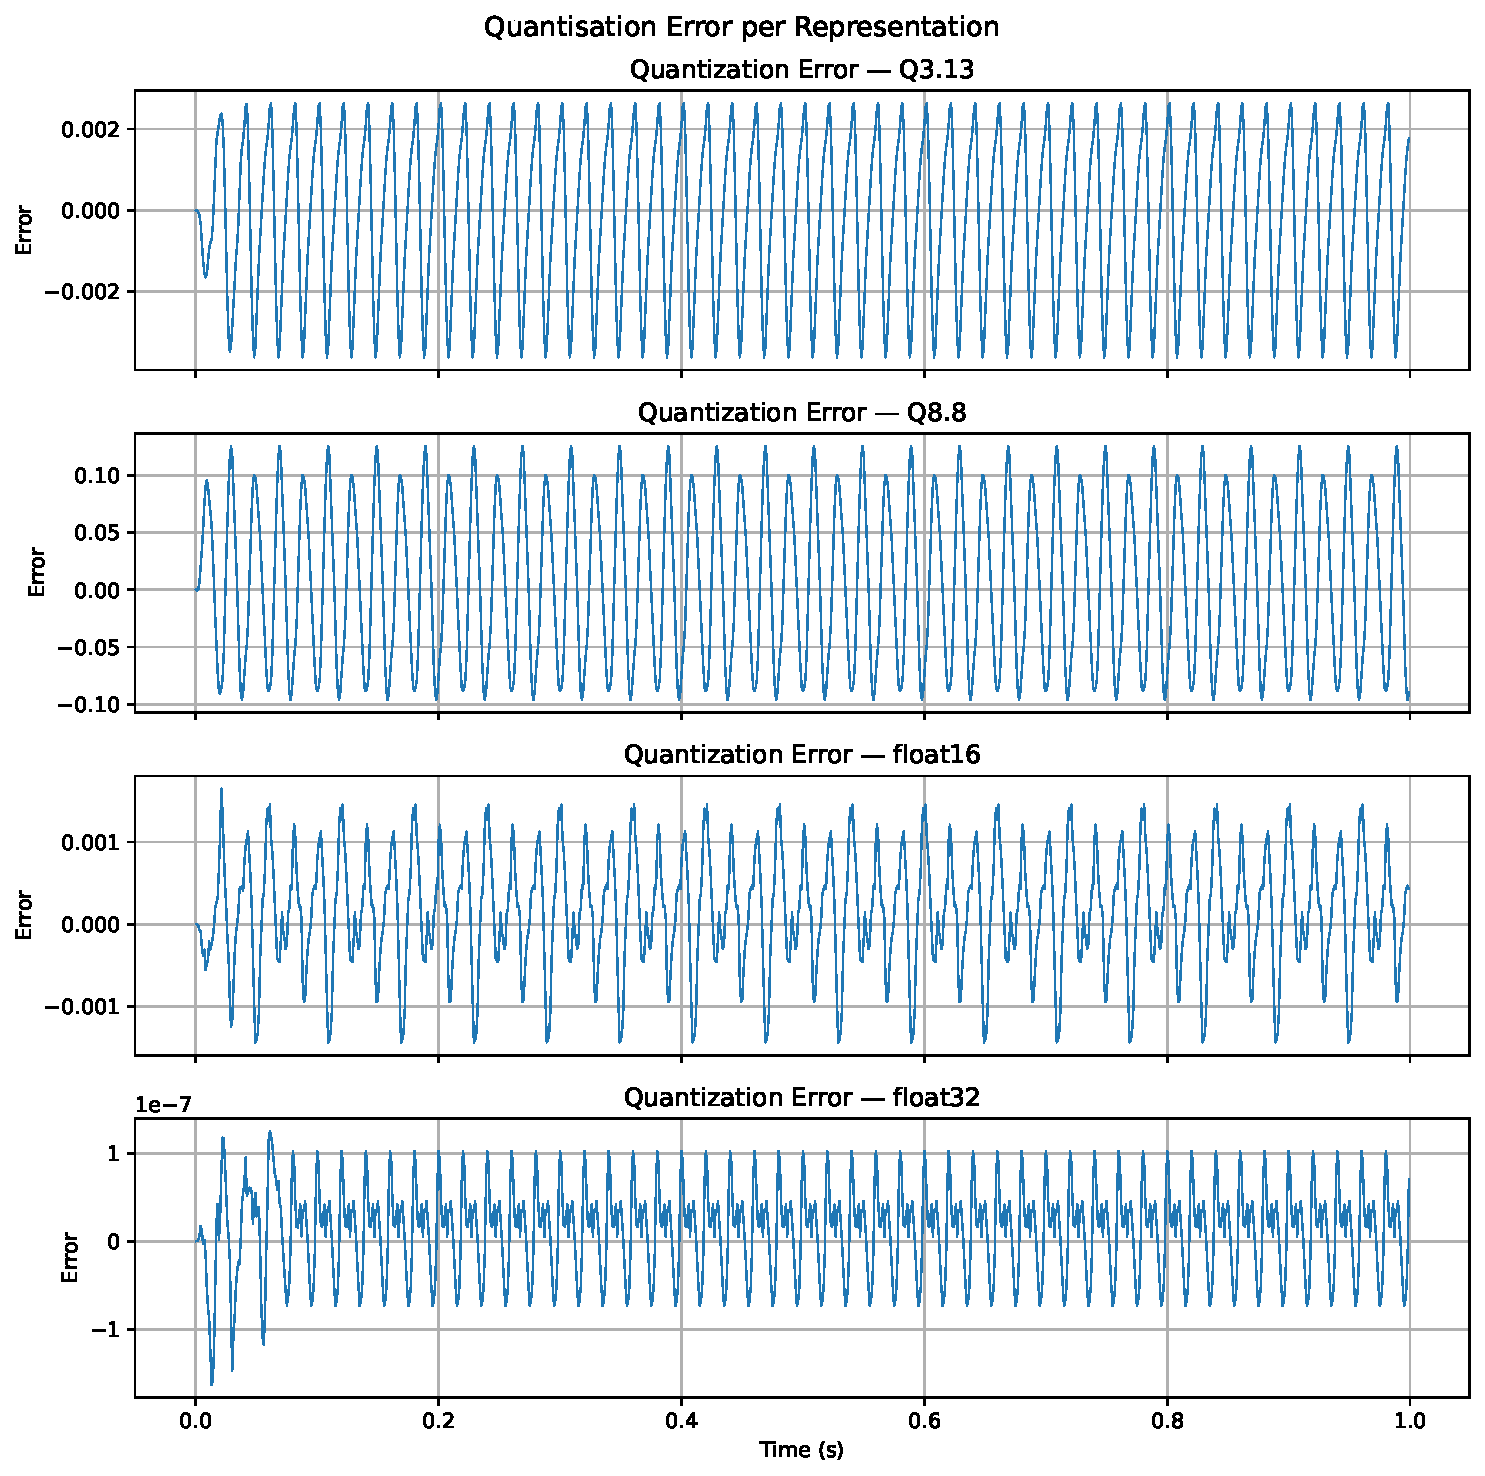
\includegraphics[width=\linewidth]{figures/error_per_format.pdf}
\caption{Per-sample quantisation error for each representation (update plot from notebook).}
\label{fig:err}
\end{figure}

Fig.~\ref{fig:hist} shows the \emph{distribution} of the same error sequence. Fixed-point histograms are wider, reflecting coarse uniform quantisation steps; float16 is intermediate; float32 concentrates tightly around zero.

\begin{figure}[htbp]
\centering
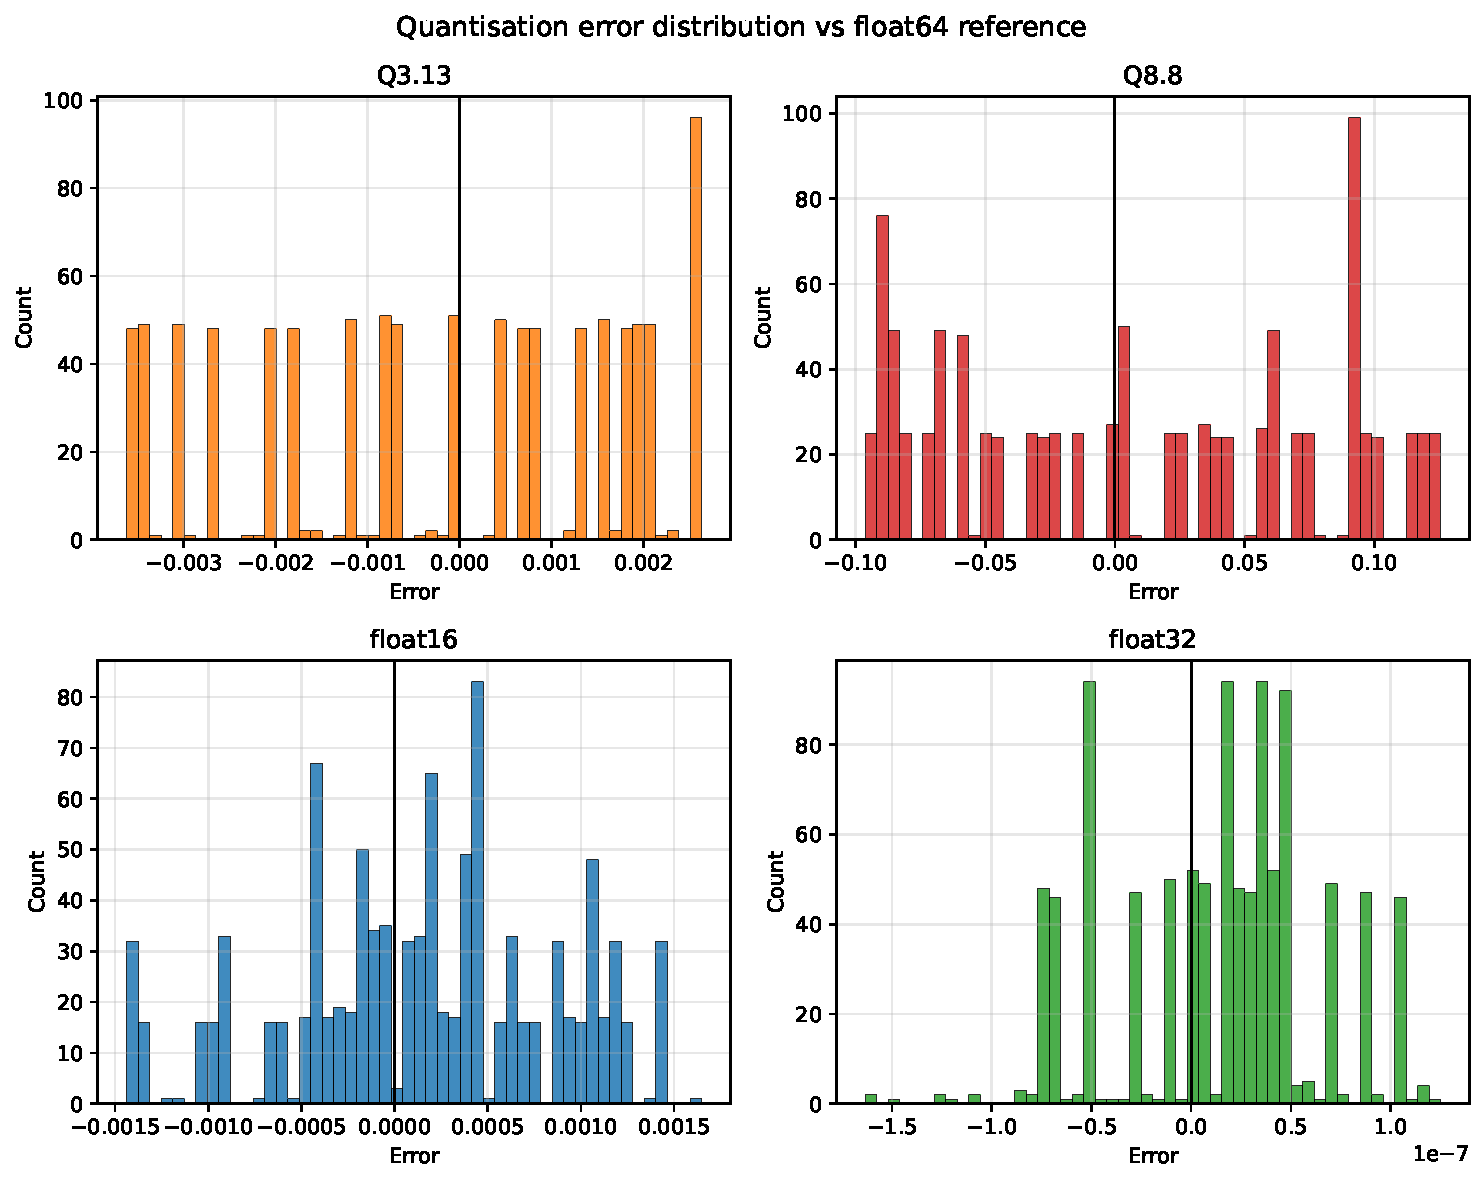
\includegraphics[width=\linewidth]{figures/error_histograms.pdf}
\caption{Histogram of $e[n]=y_{\mathrm{ref}}[n]-\hat{y}[n]$ for each representation.}
\label{fig:hist}
\end{figure}

Fig.~\ref{fig:freq} shows the frequency-response magnitude for each quantised SOS filter vs.\ the float64 reference. Q8.8 shows visible deviation in both passband and stopband.

\begin{figure}[htbp]
\centering
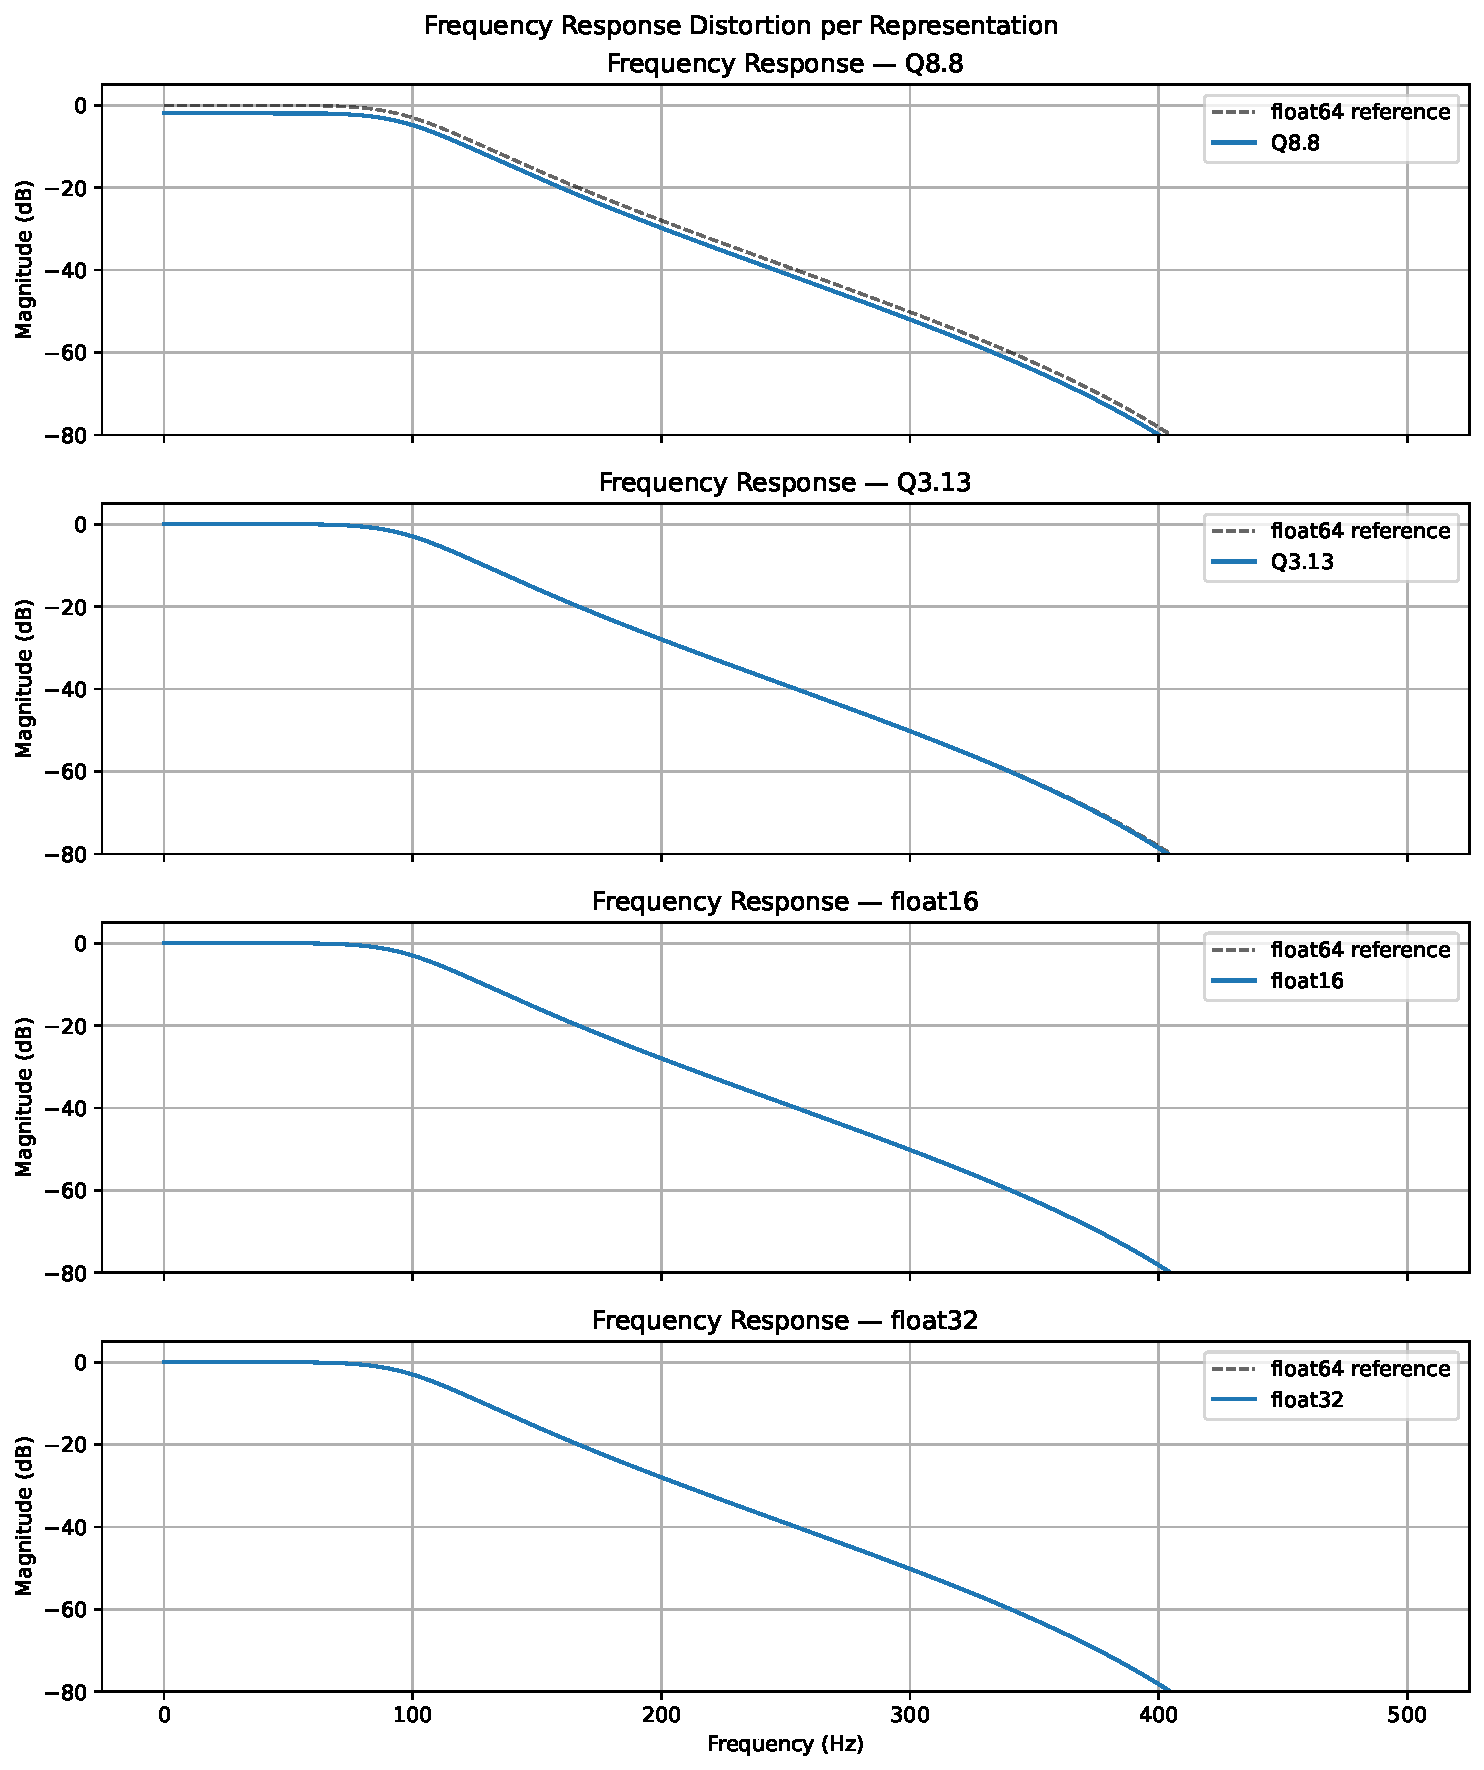
\includegraphics[width=\linewidth]{figures/freq_response.pdf}
\caption{Magnitude response vs.\ float64 reference (update from notebook).}
\label{fig:freq}
\end{figure}

Fig.~\ref{fig:snr} summarises SNR across formats.

\begin{figure}[htbp]
\centering
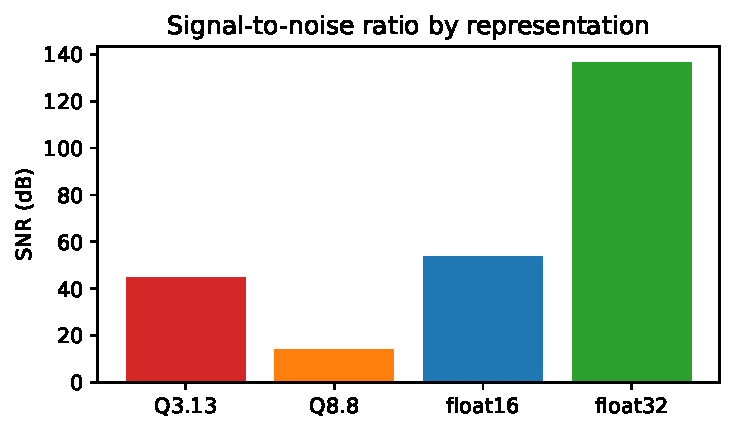
\includegraphics[width=0.85\linewidth]{figures/snr_bar.pdf}
\caption{SNR (dB) across all four representations (update from notebook).}
\label{fig:snr}
\end{figure}

\section{Discussion}

\subsection{RQ1: Characteristics, Advantages, and Disadvantages}
Fixed-point and floating-point differ along two axes: efficiency and accuracy. On efficiency, fixed-point wins for embedded targets: a 16-bit integer multiplier is smaller and more power-efficient than a 32-bit FPU; Analog Devices estimate fixed-point DSP cores cost roughly half as much and draw significantly less power~\cite{analog2007}. For battery-powered devices that is often the deciding factor. IIR filters are more sensitive to fixed-point quantisation than FIR filters because recursive feedback accumulates rounding error on every sample, whereas FIR errors are bounded by the filter length~\cite{smith1997}.

On accuracy, floating-point's adaptive exponent means precision scales with signal magnitude automatically---no manual scaling, no hard overflow for moderate signal levels. Fixed-point requires bit allocation to be decided upfront. In IIR filter design this matters because the same coefficients that define the filter's poles go through quantisation. A coarsely quantised coefficient shifts a pole's location, which changes the frequency response, as Q8.8 demonstrates in Fig.~\ref{fig:freq}~\cite{smith1997}.

The within-fixed-point comparison makes the allocation cost concrete. Q3.13 and Q8.8 use identical memory (2000~bytes) but differ by orders of magnitude in MSE. Q8.8 allocates 8 bits to an integer range ([$-128,128)$) that a normalised passband sine wave barely needs, leaving only 8 fractional bits where finer resolution is required. Q3.13 allocates 13 fractional bits---the safer match for this filter's coefficient range~\cite{ti2007}. With the corrected half-precision simulation, float16 reaches 53.68~dB SNR at 2000~bytes---higher than Q3.13 (44.87~dB) because the exponent adapts precision sample-by-sample~\cite{ieee754}, yet still far below float32.

\subsection{RQ2: Observed Quantisation Errors}
The accuracy ranking is $\mathrm{float32} \gg \mathrm{float16} > \mathrm{Q3.13} \gg \mathrm{Q8.8}$ (Table~\ref{tab:metrics}). Three observations stand out.

First, the pattern of error differs structurally between fixed and floating-point (Figs.~\ref{fig:err}--\ref{fig:hist}). Fixed-point error is periodic with roughly uniform step size; floating-point error is irregular and signal-dependent because the quantisation step scales with magnitude~\cite{smith1997}. The histograms make the spread of $e[n]$ explicit. Both are quantisation noise, but with different spectral properties relevant to audio.

Second, the frequency response (Fig.~\ref{fig:freq}) shows that Q8.8 coefficient quantisation shifts poles enough to deviate visibly from the reference. Q3.13, float16, and float32 remain close to the reference, consistent with the idea that IIR coefficient wordlength strongly shapes filter accuracy~\cite{smith1997}.

Third, float32 at 136.6~dB SNR is effectively indistinguishable from the float64 baseline for this filter. It uses twice the memory of the 16-bit formats (4000 vs.\ 2000~bytes), but on any system with an FPU it remains the appropriate default.

\section{Conclusion}
The fixed vs.\ floating-point decision is a genuine efficiency--accuracy trade-off. Fixed-point suits embedded targets without an FPU: Q3.13 achieves 44.87~dB SNR at 2000~bytes without floating-point hardware. float32 is appropriate when an FPU is present, delivering 136.6~dB SNR---effectively matching the double-precision baseline---at twice the memory of the 16-bit formats.

The more important finding remains \emph{within} fixed-point: Q8.8 and Q3.13 cost the same in memory and word length, yet Q8.8 is unsuitable for this IIR application; its large SNR deficit stems from mismatched integer vs.\ fractional bit allocation. Format selection within fixed-point is primary, not secondary. Future work should validate efficiency claims on embedded hardware (e.g., Cortex-M0 without FPU vs.\ Cortex-M4 with FPU) and extend the study to higher-order or Chebyshev filters to further stress pole sensitivity~\cite{smith1997}.

\section*{Implementation}
Code and notebooks: \url{https://github.com/YOUR_ORG/YOUR_REPO} \emph{(replace with your actual GitHub URL before submission).}

\begin{thebibliography}{00}
\bibitem{smith1997} S.~W. Smith, \emph{The Scientist and Engineer's Guide to Digital Signal Processing}, 1st ed. California Technical Publishing, 1997. ISBN 978-0-9660176-3-3. Ch.~28, ``Fixed versus Floating Point''; companion material \url{http://www.dspguide.com/ch28/4.htm} (accessed Apr.~9, 2026).

\bibitem{analog2007} Analog Devices, ``Fixed-point vs.\ floating-point digital signal processing,'' Technical Article, 2007. \url{https://www.analog.com/en/resources/technical-articles/fixedpoint-vs-floatingpoint-dsp.html} (accessed Apr.~9, 2026).

\bibitem{ti2007} G.~Frantz and R.~Simar, ``Fixed-point vs.\ floating-point digital signal processing,'' Texas Instruments, Application Rep. SPRY061, Dec.~2007. \url{https://www.ti.com/lit/wp/spry061/spry061.pdf} (accessed Apr.~9, 2026).

\bibitem{ieee754} \emph{IEEE Standard for Floating-Point Arithmetic}, IEEE Std 754-2019 (Revision of IEEE 754-2008). IEEE Standards Association, Jul.~2019. DOI: \url{https://doi.org/10.1109/IEEESTD.2019.8766229}.

\bibitem{goldberg1991} D.~Goldberg, ``What every computer scientist should know about floating-point arithmetic,'' \emph{ACM Computing Surveys}, vol.~23, no.~1, pp.~5--48, Mar.~1991. DOI: \url{https://doi.org/10.1145/103162.103163}.

\bibitem{oppenheim2010} A.~V. Oppenheim and R.~W. Schafer, \emph{Discrete-Time Signal Processing}, 3rd ed. Upper Saddle River, NJ, USA: Pearson, 2010. ISBN 978-0-13-198842-2.

\bibitem{spfpm} R.~W. Penney, \emph{SPFPM: Simple Python Fixed-Point Module} (software), GitHub repository. \url{https://github.com/rwpenney/spfpm} (accessed Apr.~9, 2026). Pin the release tag or commit SHA in your report if your module requires reproducibility beyond ``main''.

\bibitem{scipy2020} P.~Virtanen \emph{et al.}, ``SciPy 1.0: Fundamental algorithms for scientific computing in Python,'' \emph{Nature Methods}, vol.~17, no.~3, pp.~261--272, Mar.~2020. DOI: \url{https://doi.org/10.1038/s41592-019-0686-2}.

\bibitem{harris2020} C.~R. Harris \emph{et al.}, ``Array programming with NumPy,'' \emph{Nature}, vol.~585, pp.~357--362, Sep.~2020. DOI: \url{https://doi.org/10.1038/s41586-020-2649-2}.

\end{thebibliography}

\end{document}
